\documentclass{../../text-style}

\texttitle{Лекция 13: Проектирование распределённых приложений, стратегические вопросы}

\begin{document}

\maketitle
\thispagestyle{empty}

\section{Архитектурные стили распределённых систем}

В этой лекции поговорим о <<стратегических>> аспектах проектирования распределённых (прежде всего, больших облачных) приложений. Начнём с типичных для них архитектурных стилей. Все они в целом строятся либо согласно слоистому стилю, либо согласно разным подвидам событийно-ориентированного стиля, однако в реальной жизни используются обычно более специфичные стили, о них-то и поговорим.

Далее архитектурные стили упорядочены по возрастанию <<обычности>> для современных облачных приложений (по крайней мере, по мнению автора). Изложение ведётся в основном по архитектурным гайдлайнам платформы Microsoft Azure\footnote{Azure Architecture Center, URL: \url{https://docs.microsoft.com/en-us/azure/architecture/} (дата обращения: 11.12.2021).} с аккуратно вырезанными вендор-специфичными штуками, тем не менее, данный обзор не претендует на полноту.

\subsection{Big Compute}

Архитектурный стиль <<Большие вычисления>> (<<Big Compute>>) предназначен для решения задач, требующих массовой параллельности. Лекционный курс <<Параллельное программирование>> на матмехе, как говорят, начинается со слов <<представим, что у нас есть компьютер с бесконечным количеством процессоров, посмотрим, что на нём можно посчитать>> --- это и есть типовая ситуация применения Big Compute. Типичные задачи, решаемые в таком стиле --- это прежде всего физические или химические расчёты, симуляция, различного рода моделирование, решение огромных дифуров и т.п., то есть задачи, которыми на матмехе активно занимается кафедра параллельных алгоритмов, и которые обычно требуют суперкомпьютер. 

Архитектурно подобные системы устроены довольно просто:

\begin{center}
    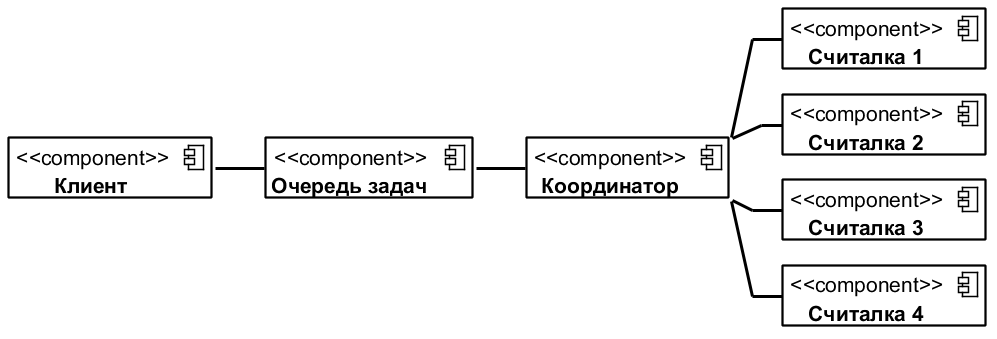
\includegraphics[width=0.8\textwidth]{bigCompute.png}
\end{center}

Есть клиент, снабжающий систему данными и запросами, есть очередь задач, куда запросы попадают от клиента, и есть координатор (на самом деле, самая сложная часть системы), который берёт задачи из очереди, делит на подзадачи и раскидывает по вычислительным узлам. Каждый вычислительный узел обычно устроен довольно просто, но интересно то, что их много --- от десятков до десятков тысяч. При этом вычисления бывают хорошо параллелизуемыми (в идеале --- представимыми в виде Map-Reduce-вычисления), тогда части задачи можно раскидать по узлам и они могут считать, никак не координируясь друг с другом. Когда все узлы закончат обработку, координатор собирает результаты, агрегирует их (возможно, задействуя ещё узлы) и выдаёт ответ. В этом случае каждый узел должен обладать большими ресурсами (прежде всего, процессором, но может потребоваться и оперативная память), но требований к сети почти нет.

Бывают, однако, параллельные задачи, требующие активной координации между узлами. В этом случае требуется также высокопроизводительная сеть, и тогда вычислительные узлы по сути соединены в вычислительный кластер, хоть и могут физически предоставляться облачным провайдером просто из каких-то доступных ресурсов.

Этот архитектурный стиль довольно специфичен, поскольку вычислительно сложные задачи в современном мире относительно редки (зато если вы умеете такое делать, можете просить любую зарплату --- для этого на матмехе и учат дифурам и матфизике). Кроме того, требуется <<embarrassingly parallel>>-задача (что обычно переводится на русский как <<чрезвычайно параллельная>>, но английский термин более точен --- настолько параллельная, что даже стыдно), иначе выгоды от параллелизма будет немного. Кроме того, требуются весьма продвинутые и дорогие ресурсы, которые у современных провайдеров облачной инфраструктуры типа AWS или Azure, конечно, есть, но стоить их аренда будет немало (а купить себе небольшой суперкомпьютер и содержать его будет ещё в разы дороже). Однако для таких задач зачастую просто не существует других способов решения, кроме как грубой силой.

\subsection{Big Data}

Всеми любимые большие данные --- это обратная сторона Big Compute, когда вычисления не сложны, просто их очень много. Архитектурный стиль для обработки этих данных применяется, когда они не лезут в обычную СУБД, и структурно на самом деле похож на Big Compute, особенно если данные надо обрабатывать <<на лету>>:

\begin{center}                                                                                 
    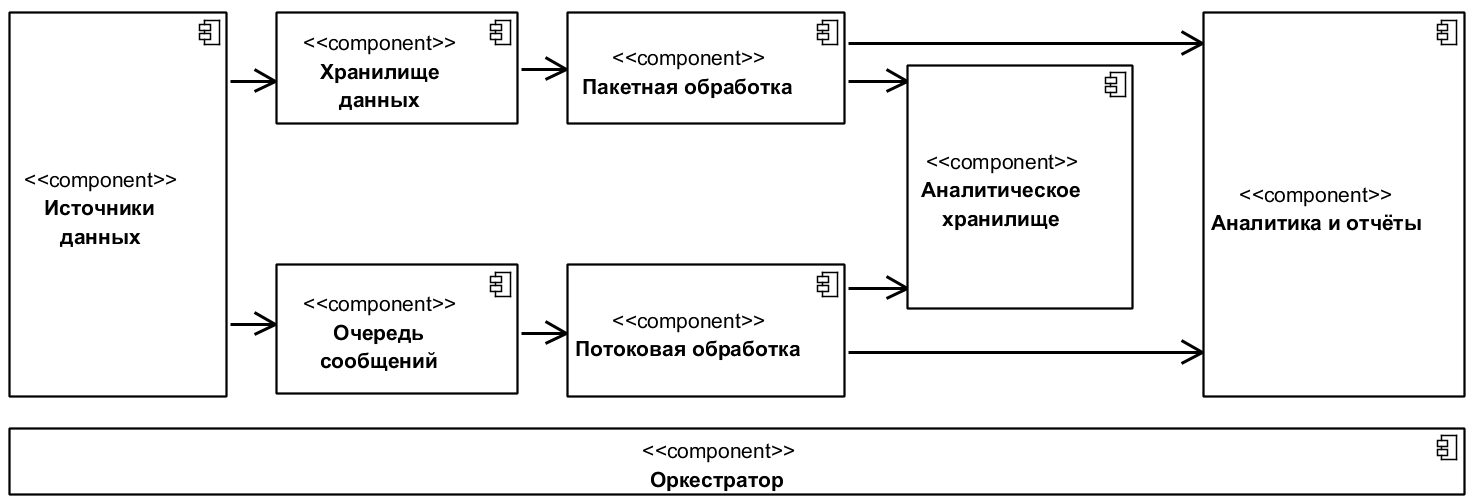
\includegraphics[width=0.9\textwidth]{bigData.png}
\end{center}

В любом случае, данные поступают в систему извне, из какого-либо источника (обычно многих разных), где они могут быть представлены в виде, не очень пригодном для обработки, поэтому надо их сначала импортировать. Дальше возможны два варианта:

\begin{itemize}
    \item данные надо обрабатывать на лету --- например, банковские транзакции или показания датчиков; тогда они обычно все кидаются в очередь сообщений (например, Apache Kafka), откуда их параллельно вычитывает несколько потоковых обработчиков (очередь служит и буфером, и балансировщиком нагрузки), обработанные данные попадают в аналитическое хранилище для дальнейшей работы с ними или в отчёты, выдаваемые пользователю (или другим системам);
    \item данные можно обрабатывать с регулярными интервалами --- например, формировать сводки за день; тогда вместо очереди сообщений может использоваться распределённое хранилище, куда данные импортируются из источников, и оттуда они время от времени вычитываются обработчиками (опять-таки, возможно, параллельно).
\end{itemize}

Поскольку данных заведомо много, требуются механизмы их распределённого хранения и обработки. Писать их с нуля крайне не рекомендуется, потому что простую систему написать, конечно, можно быстро, но как только появляются требования оптимальности загрузки ресурсов, отказоустойчивости и безопасности, внезапно начинает требоваться продвинутая математическая и алгоритмическая теория, которую лучше доверить профессионалам. Примеры готовых решений --- Apache Hadoop (с его распределённой системой хранения данных HDFS и распределённой системой обработки MapReduce), Apache Spark (который поновее и побыстрее за счёт хранения данных в памяти). Hadoop хорош для пакетной обработки, Spark тяжелее в настройке и эксплуатации, но хорош для обработки в реальном времени.

Хранение данных тоже не так просто. В традиционных СУБД данные должны соответствовать некоторой схеме, чтобы их можно было даже хранить, однако архитектурный стиль <<Big Data>> говорит, что это плохо --- необходимость конвертации к единому формату может переусложнить систему и потенциально стать узким местом в плане производительности. Поэтому рекомендуют пользоваться принципом Schema-on-read --- хранить данные в том виде, в котором они пришли (сырые логи, текстовые документы, таблицы и т.п.), и преобразовывать их в нужный формат уже при чтении для обработки. Это позволит разным обработчикам использовать разные форматы, при этом пользуясь одним общим распределённым хранилищем данных. Для такого хранилища слабоструктурированных или неструктурированных данных есть модный термин <<Data Lake>>, и ему часто противопоставляют термин <<Data Swamp>> --- когда данные в хранилище есть, но никто не знает, как ими пользоваться, чтобы извлечь что-то полезное.

Вполне возможно, что хранилище данных само может обеспечить предварительную обработку данных (фильтрацию, преобразование, некоторую агрегацию), тогда этим надо пользоваться. Традиционный подход к обработке данных --- Extract, Transform, Load (ETL), вместо этого рекомендуется схема Transform, Extract, Load (то есть обработка на стороне хранилища --- того же Apache Hadoop, извлечение обработанных данных и загрузка их в аланитическое хранилище).

Если обработка выполняется в пакетном режиме, полезный приём --- это делить входные данные по интервалам обработки. Например, если метрики считаются по логам раз в день, настройте систему логирования так, чтобы она раз в день делала ротацию логов\footnote{Общая практика для систем логирования, когда по достижению определённого размера или прошествию определённого времени лог архивируется и на его месте заводится новый. Например, log4j и log4net так, конечно, умеют --- см. RollingFileAppender.}, и отправляйте на обработку как раз тот кусок данных, который должен быть обработан за один раз. Это несколько упрощает анализ и, если что-то пойдёт не так, упрощает локализацию проблемы.

Ещё один важный практический совет --- если считается какая-то агрегатная статистика, личные данные должны удаляться как можно раньше (в идеале --- никогда не покидать сам источник данных). Несмотря на все усилия по обеспечению безопасности, данные украдут, и если от этого никто не пострадает, все будут только в выигрыше.

Вот пример применения такого подхода, типичная архитектура систем <<интернета вещей>>:

\begin{center}
    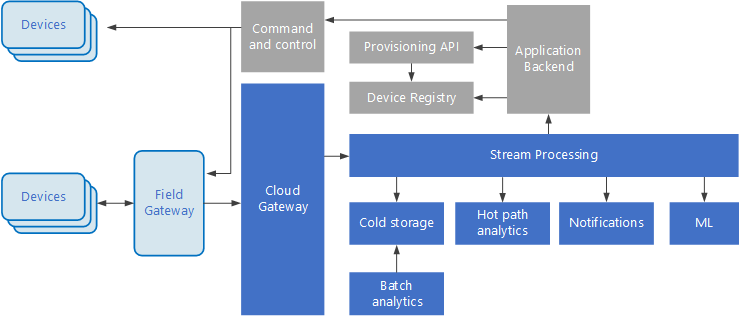
\includegraphics[width=0.9\textwidth]{iot.png}
    \attribution{https://github.com/MicrosoftDocs/architecture-center/blob/main/docs/guide/architecture-styles/big-data.md}
\end{center}

Устройства (например, охранные датчики, медицинские устройства) передают свои показания на Field Gateway (располагающийся близко к самим устройствам), он выполняет базовую обработку и агрегацию и отправляет данные на Cloud Gateway, находящийся уже в центре обработки данных (если каждое устройство будет слать свои показания прямо в облако, даже облако с этим может не справиться, ну или это будет стоить сказочных денег). Оттуда данные попадают в систему потоковой обработки, которая может делать разные вещи --- сохранять данные в <<холодное хранилище>> для последующей пакетной обработки (считать разные статистики, например), анализ в реальном времени, посылать нотификации или скармливать данные разным алгоритмам машинного обучения (например, для детекции аномалий).

Также возможно, хотя и не обязательно, что есть и обратный поток, от облака к устройствам (показано серым на диаграмме). Результаты потоковой обработки попадают в бэкенд, который передаёт команды управления на устройства (возможно, опять-таки через Field Gateway). К тому же, бэкенд отвечает за регистрацию новых устройств и хранение информации об устройствах.

\subsection{Событийно-ориентированная архитектура}

Событийно-ориентированный стиль, конечно, также применяется для обработки данных в распределённых (в т.ч. облачных) системах. Однако в силу принципиальной ненадёжности сети издатель и подписчики редко связаны напрямую, между ними обычно находится событийная шина. В событийную шину может писать сколько угодно издателей и обработкой событий оттуда может заниматься сколько угодно подписчиков. Стиль архитектурно простой, и существующие решения позволяют сделать такие системы очень производительными, поэтому он часто применяется для обработки событий в реальном времени:

\begin{center}
    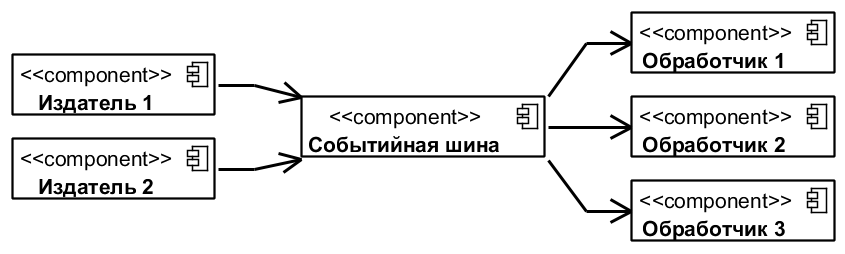
\includegraphics[width=0.7\textwidth]{eventDrivenArchitecture.png}
\end{center}

Принципиально моделей обработки событий две.

\begin{itemize}
    \item Издатель/подписчик --- когда сообщение попадает в шину, его забирает и обрабатывает один из подписчиков. В качестве шины может выступать очередь сообщений, имеющая такую семантику, например, RabbitMQ (хотя надо понимать, что их бывает много, например, ZeroMQ более легковесна и поэтому может с успехом применяться в IoT).
    \item Event Sourcing --- когда сообщение попадает в шину и остаётся там навсегда, чтобы кому надо могли прочитать его и обработать --- в том числе, вновь подключившийся клиент всегда может проиграть всю историю сообщений с начала, чтобы получить текущую картину мира. Тут в качестве шины могут выступать распределённые логи событий, например, Apache Kafka (хоть они могут быть внешне неотличимы от очередей сообщений). Для быстрой потоковой обработки это считается более прогрессивным подходом, потому что требует меньше координации между участниками взаимодействия и работает быстрее. В этом случае обычно текущее состояние системы в явном виде не хранится, или хранится в виде снапшотов, которые не являются источником истины, а всего лишь ускоряют доступ (то есть реализуется принцип eventual consistency --- каждый обработчик может иметь свою картину мира, немного запаздывающую во времени, но рано или поздно все всё вычитают и узнают).
\end{itemize}

\subsection{Web-queue-worker}

Web-queue-worker --- это некое уточнение событийно-ориентированного стиля, применяемое прежде всего для вычислительно сложных задач, если предметная область относительно несложна и не требует детального моделирования (пакетная обработка каких-то данных, например, типа конвертации pdf-документов). Поскольку это уже <<приближенный к земле>> стиль разработки веб-приложений, его структура более детальна:

\begin{center}
    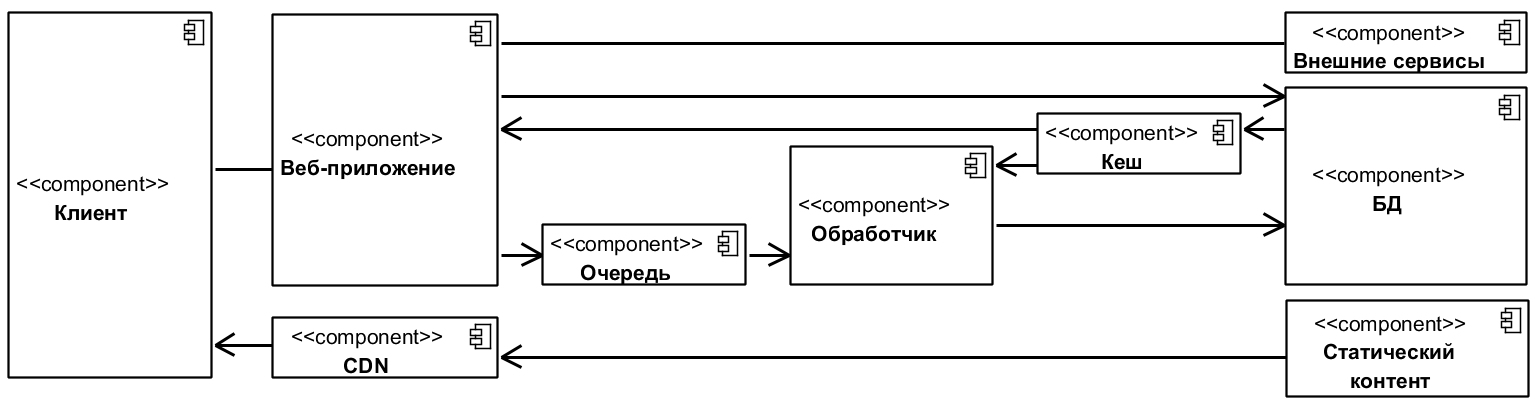
\includegraphics[width=0.9\textwidth]{webQueueWorker.png}
\end{center}

\emph{Клиент} работает в браузере у пользователя, через него пользователь заказывает выполнение работы. \emph{Веб-приложение} на стороне сервера поддерживает действия клиента, и принимает от него работу. Задания вместе с необходимыми данными попадают в \emph{очередь}, откуда вычитываются \emph{обработчиками}. Результаты обработки сохраняются в \emph{базу данных}, откуда, возможно, через \emph{кеш} читаются веб-приложением (и обработчиками, если им нужны данные из базы). При этом веб-приложение может пользоваться также \emph{внешними веб-сервисами}, а клиент --- получать \emph{статический контент} (картинки, скрипты, стили, файлы) через \emph{Content Delivery Network}.

Удивительно, но очередь и обработчик в такой схеме не обязательны --- если сложных вычислений нет, всё может делаться самим веб-приложением (и тогда это будет обычной трёхзвенной архитектурой). Однако если надо что-то сложное считать, то очередь очень полезна, поскольку работает буфером, смягчающим эффекты пиковой нагрузки, да ещё и балансировщиком. При этом разделение обработчика и веб-части позволяет масштабировать их независимо, так что если фронт справляется, а вычислительно сложная часть нет, можно отдельно поднять ещё несколько обработчиков, и остановить их, когда в них пропадёт нужда. Обратите внимание, что запросы принципиально выполняются асинхронно, то есть заставлять пользователя ждать, пока придёт ответ, тут пагубная практика.

Кроме того, такая архитектура позволяет эффективно использовать уже готовые технологии --- например, веб-приложение на ASP.NET или Spring, очередь RabbitMQ, обработчик в виде веб-сервиса на том же ASP.NET, читающего из очереди, MariaDB в качестве БД и Redis в качестве кеша. При этом можно использовать готовые CDN для, например, React и стилей Bootstrap. Если знать, что делать, собрать такую штуку можно за выходные, почему Web-Queue-Worker и популярен в продакшене.

Однако за всё надо платить, при росте сложности предметной области начинает разрастаться либо веб-часть, либо обработчик, либо и то и другое. Очень легко пропустить тот момент, когда такое приложение превратится в большой бесформенный клубок кода, который невозможно больше поддерживать. В этом случае поможет более аккуратная декомпозиция ответственности, предполагаемая следующими архитектурными стилями.

\subsection{N-звенная архитектура}

Знаменитая N-звенная архитектура, разумеется, в облачных приложениях тоже вполне используется: 

\begin{center}
    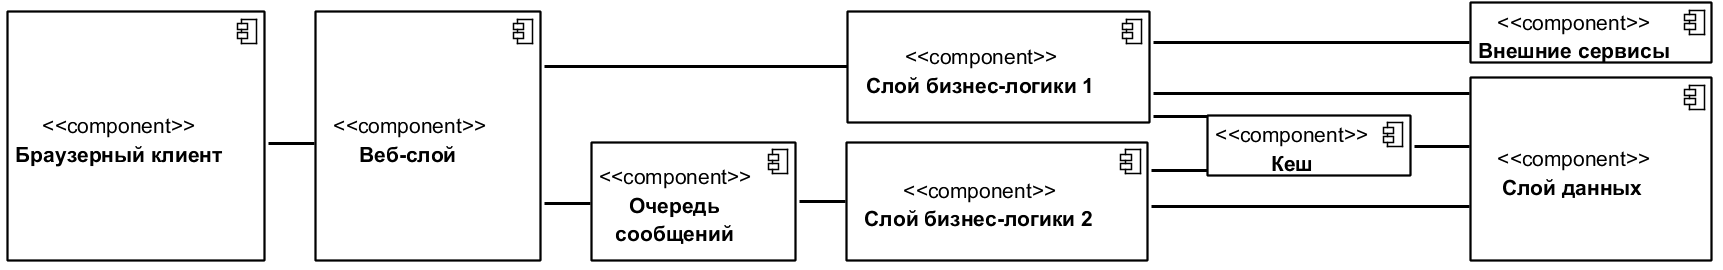
\includegraphics[width=0.9\textwidth]{nTierArchitecture.png}
\end{center}

\emph{Браузерный клиент}, что не удивительно, работает в браузере у пользователя (это может быть одностраничное приложение на чём-нибудь вроде React bли Vue, может быть и многостраничное на каком-нибудь из серверных веб-фреймворков). \emph{Веб-слой} поддерживает клиентское приложение и, возможно, обрабатывает асинхронные запросы. Веб-слой общается со слоем \emph{бизнес-логики}, который может быть сколь угодно сложно устроен (например, как на рисунке, их может быть два, и один из них подключен через очередь сообщений, но это не требование стиля, а только пример). Слой бизнес-логики общается с \emph{внешними сервисами} и \emph{слоем данных}, при этом слой данных может быть доступен на чтение через кеш (если это повысит производительность, конечно). Особенностью этого стиля является то, что компоненты приложения обычно физически размещаются на разных машинах, что помогает в масштабируемости и надёжности.

Такой архитектурный стиль хорош, когда у вас уже есть монолитное приложение, работающее на вашем любимом сервере, и вы хотите с минимумом трудозатрат перенести его куда-нибудь на AWS. Либо бизнес-логика несложная (но всё же требует некоторой структуризации, так что Web-Queue-Worker не подойдёт). Однако масштабировать при таком подходе можно только крупные куски системы, так что если ваша бизнес-логика содержит два метода, одним из которых никто никогда не пользуется, а один не справляется с нагрузкой, вы должны запустить второй экземпляр сервера бизнес-логики целиком. Ещё, как обычно, слой бизнес-логики имеет тенденцию разрастаться и превращаться в большой ком грязи.

Вот пример типичного N-звенного веб-приложения на Azure, использующего стек технологий от Microsoft:

\begin{center}
    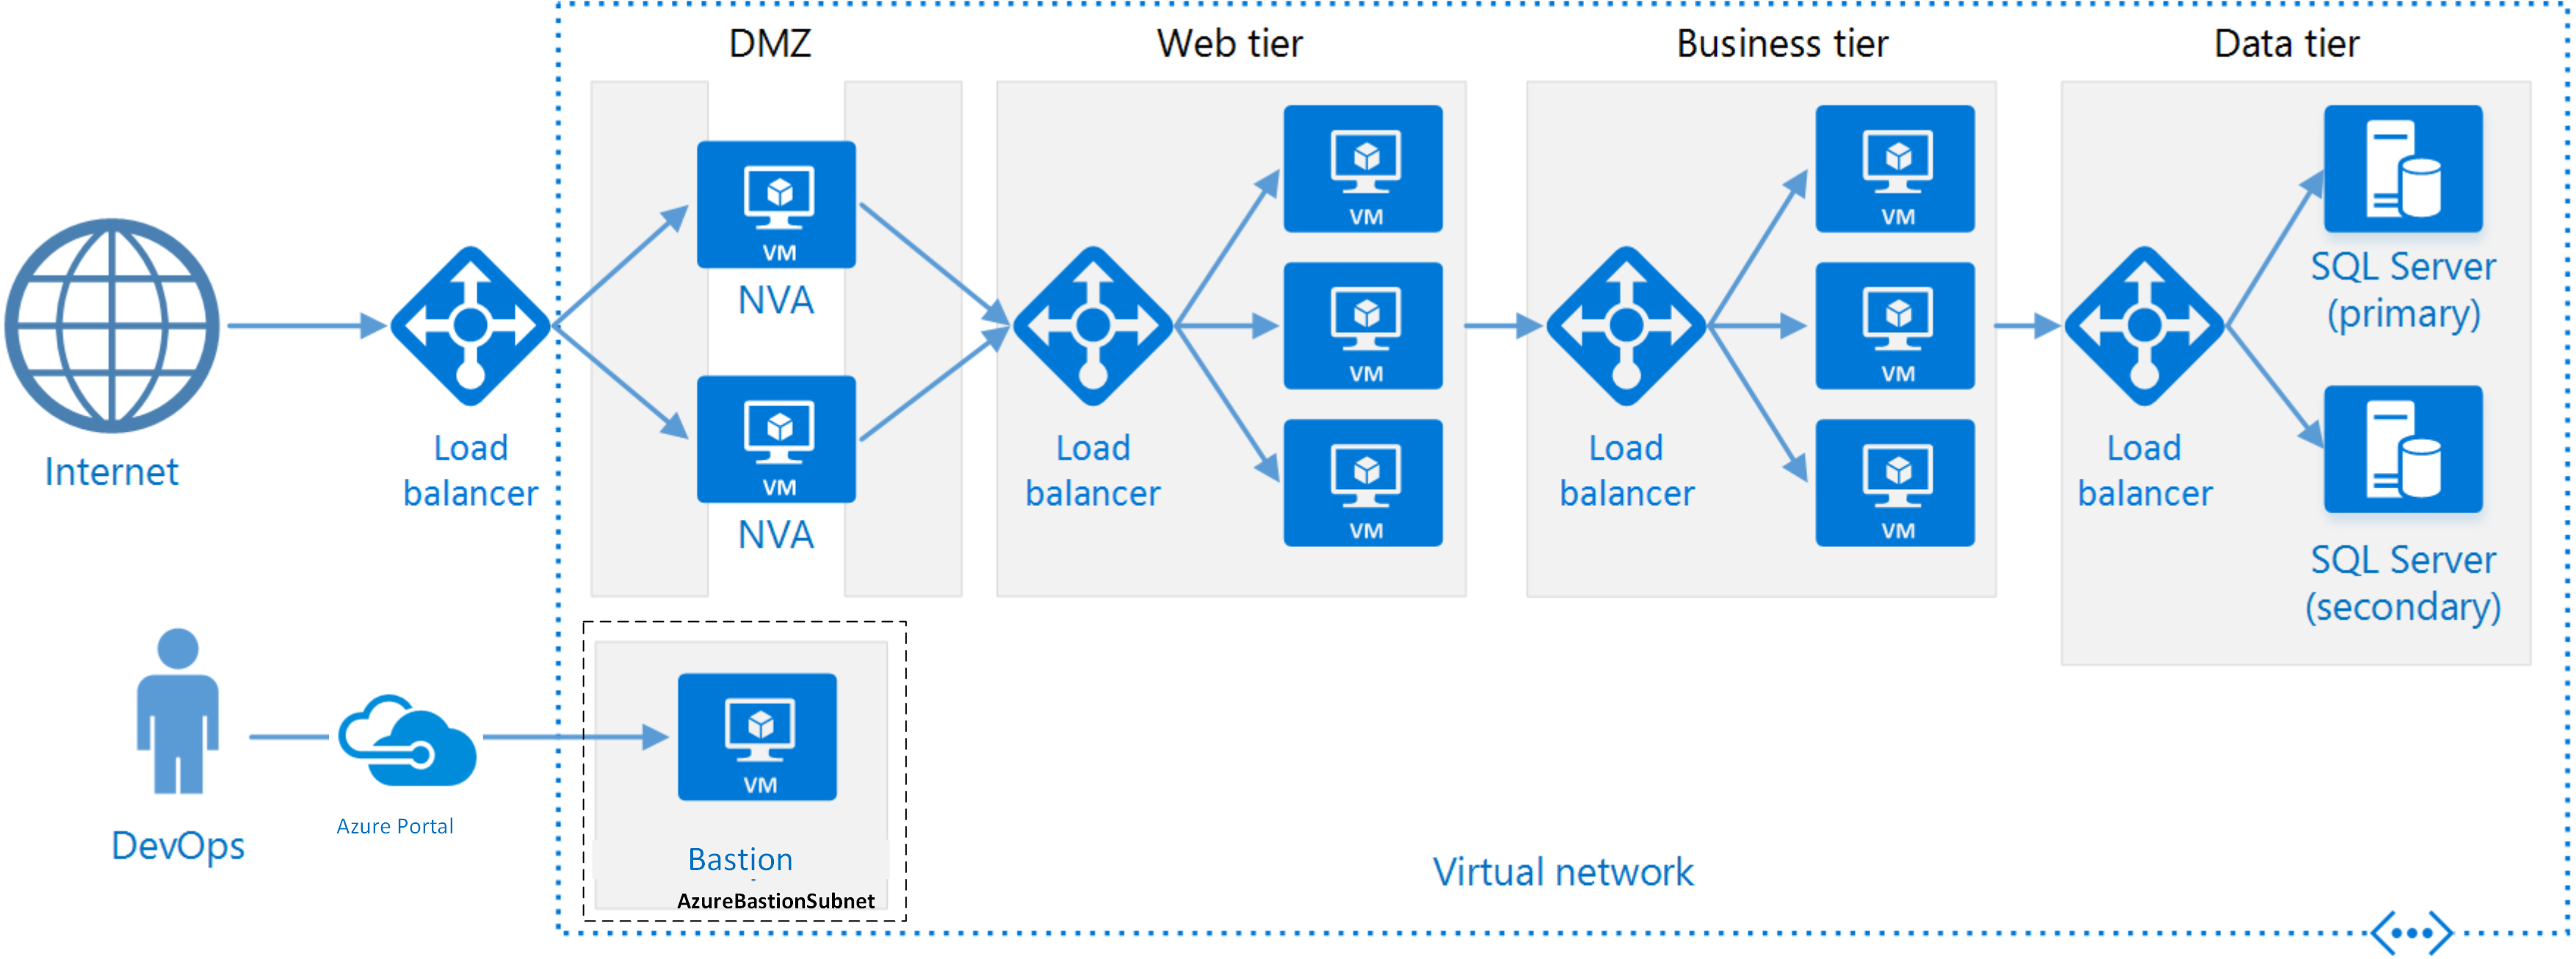
\includegraphics[width=\textwidth]{n-tier-physical-bastion.png}
    \attribution{https://github.com/MicrosoftDocs/architecture-center/blob/main/docs/guide/architecture-styles/n-tier.md}
\end{center}

На входе стоит балансировщик нагрузки, перекидывающий запросы на сервера Network Virtual Appliances внутри Demilitarized Zone, обеспечивающие безопасность (инспекцию пакетов, файерволл и т.п.). Это всё готовые компоненты, которые надо просто подключить к инфраструктуре. Всё остальное происходит внутри виртуальной сети, доступа к машинам которой снаружи нет (есть ещё админский доступ через Bastion --- по сути, ssh-сервер, с которого после прохождения всей необходимой авторизации можно ходить на другие машины в виртуальной сети). За DMZ находится пул виртуальных машин веб-части, за которым --- пул виртуалов бизнес-части, за которым --- кластер с СУБД (который может заниматься просто репликацией, тогда балансировщик нагрузки единственное, что делает --- переключает на горячую копию, если основная СУБД померла; а может заниматься продвинутым шардированием, о чём чуть позже). 

Каждый из слоёв системы состоит из виртуальных машин за балансировщиком нагрузки --- во-первых, для повышения производительности, во-вторых, для надёжности (если одна машина умрёт, балансировщик просто не будет направлять ей запросы, так что её смерть никто извне не заметит), в-третьих, для масштабируемости. Изначально в пуле может быть только одна виртуалка, но если она перестаёт справляться, может динамически запускаться вторая и брать на себя работу с помощью балансировщика. Запускать новую машину в пуле можно руками, а можно и автоматически, при достижении критического значения какой-то из метрик (например, загружености процессора выше 80\%), для чего облачные провайдеры имеют развитые средства мониторинга состояния виртуальных машин.

С инфраструктурой, тем более её автоматическим масштабированием, однако, надо быть осторожными, поскольку аренда виртуальных машин и прочих штук типа балансировщиков нагрузки, стоит денег, и иногда немалых. Сначала следует определиться с бизнес-целями --- принесёт ли обеспечение дополнительной надёжности и производительности приложения достаточно денег, чтобы покрыть расходы на инфраструктуру.

\subsection{Микросервисная архитектура}

Микросервисная архитектура на данный момент самая популярная для распределённых приложений, хотя архитектурная мода как маятник раскачивается между микросервисными и монолитными приложениями. Микросервисный подход предлагает делить приложение на маленькие куски, каждый из которых представляет собой отдельный веб-сервис и достаточно мал по размеру, чтобы его <<мог написать один человек за две недели>> (на самом деле, в реальной жизни микросервисы обычно побольше --- подходящего размера, чтобы один микросервис могла разработать и сопровождать одна небольшая команда, но зависит от конкретного проекта, конечно). Микросервис имеет свою модель предметной области и является ограниченным контекстом с точки зрения предметно-ориентированного проектирования. Итоговое приложение собирается из микросервисов, вызывающих друг друга:

\begin{center}
    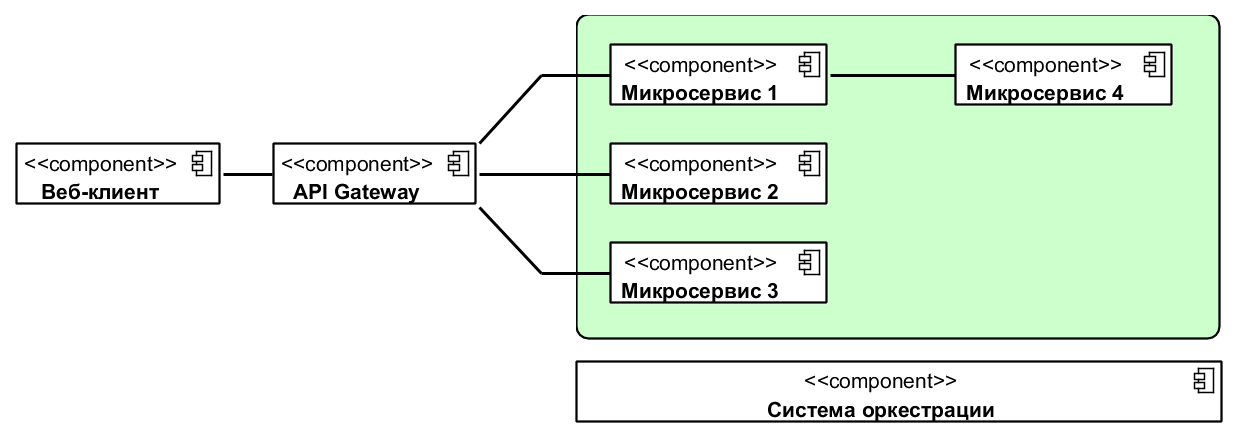
\includegraphics[width=0.85\textwidth]{microservices.png}
\end{center}

Как обычно, есть \emph{веб-клиент}, который шлёт запросы на \emph{API Gateway}. Также вполне может быть и выделенная веб-серверная часть, а может и не быть --- отдаваемая клиенту страница может собираться из элементов, предоставляемых отдельно каждым микросервисом. Gateway не содержит никакой бизнес-логики, а просто перенаправляет запросы внутрь виртуальной сети, где работают микросервисы, и нужен прежде всего для того, чтобы у клиента был один фасад для всего приложения, и ему не надо было знать адреса отдельных частей. \emph{Система оркестрации} (например, Docker Compose или Kubernetes) управляет временем жизни микросервисов, масштабированием, балансировкой нагрузки, мониторингом и т.п. --- для микросервисных приложений это на самом деле очень важная вещь, поскольку сложность системы во многом определяется не реализацией самих микросервисов, а связями между ними.

Этот архитектурный стиль успешно применяется для предметных областей произвольной сложности (начиная с небольших приложений наподобие HwProj 2, где микросервисов меньше десятка, заканчивая гигантскими системами типа Facebook, c сотнями разных микросервисов).

Особенности микросервисного подхода таковы:

\begin{itemize}
    \item Поскольку каждый микросервис --- это отдельное приложение, он может быть написан на своём языке и стеке технологий, независимо от других. Хорошо это или плохо, открытый вопрос, потому что с одной стороны, это позволяет каждому писать на языке, на котором он наиболее продуктивен, с другой стороны, зоопарк из технологий усложняет поддержание инфраструктуры разработки. Но поскольку любой сервис можно переписать за две недели, это не то чтобы большая проблема.
    \item Каждый микросервис хранит свои данные сам, не имеет право разделять схему данных с другими. В этом смысле микросервис схож с объектом из классического ООП, то есть имеет своё внутреннее состояние и внешнее поведение. Обмениваться данными с другими микросервисами, конечно, можно, но только через публичный интерфейс. Это позволяет микросервисам выбирать наиболее эффективные способы хранения данных --- не требуется поднимать один на всё приложение настоящий сервер с СУБД, как в N-звенной архитектуре, можно обойтись легковесными решениями типа SQLite или выбрать подходящую NoSQL-базу (но помните про масштабирование, все реплики одного микросервиса должны быть согласованы --- проще всего это обеспечить, если сам микросервис состояния не имеет вовсе, но можно иметь СУБД, на которую смотрят все реплики).
    \item Каждый микросервис может быть масштабирован независимо, причём это делают даже не специальные балансировщики нагрузки, как в случае с N-звенной архитектурой, а сами оркестраторы, которые всё равно нужны и всё равно всем управляют. Так что если у вас есть функция, которая никому не нужна, запустите одну реплику с ней и пусть будет, и если есть функция, которая не справляется со своей работой, запустите хоть десять реплик только для неё. Микросервисы обычно работают в контейнерах, а не на виртуальных машинах, так что это ещё и дешевле, если делается на арендованных облачных мощностях.
    \item Каждый микросервис может быть задеплоен независимо от остальных, если его внешний интерфейс не менялся, так что циклы разработки и релизы отдельных микросервисов не должны быть согласованы. В отличие от монолита, где один маленький баг может задерживать релиз всей системы. ДАже если внешние интерфейсы менялись, согласовывать развёртывание надо только с соседними командами, а не со всем проектом. Поэтому микросервисные системы могут позволить себе по несколько релизов \emph{в день} и даже подход <<любой коммит сразу в production>>.
    \item Каждый микросервис падает отдельно, так что если вся система написана с расчётом на то, что любой компонент может отказать, любой сбой может быть легко локализован и не приведёт (по идее) к отказу всей системы.
    \item Микросервисы на то и микро, чтобы кодовая база каждого была очень маленькой и простой, что позитивно сказывается на стоимости сопровождения.
\end{itemize}

Однако, конечно, за всё надо платить. У микросервисного архитектурного стиля достаточно и недостатков. Прежде всего то, что сложность приложения перекладывается с кода на оркестрацию. А это не очень хорошо, потому что языки и приёмы программирования эволюционируют уже почти столетие, а технологии для конфигурирования взаимодействия микросервисов, в целом, только в начале пути. Так что зависимости между микросервисами могут быть неочевидны, их трудно отлаживать и мониторить, требуется набор специальных знаний и навыков, развитая культура DevOps во всей организации. Кроме того, само по себе микросервисное приложение сложнее эквивалентного по функциональности приложения в других стилях, в силу большего оверхеда на всякие инфраструктурные задачи. Да и разработка/тестирование сложнее, поскольку требуется либо куча mock-объектов, либо умение быстро поднимать и запускать все зависимости.

Кроме того, микросервисные приложения гораздо более требовательны к сетевой инфраструктуре, поскольку куча вызовов, которые в других стилях делаются локально, в микросервисном стиле сетевые (поэтому, кстати, не получится взять монолит и сделать каждый класс микросервисом --- сеть ляжет). Обычно все микросервисы находятся внутри одной сети облачного провайдера, и там могут применяться очень скоростные соединения (например, InfiniBand, где скорость передачи измеряется в сотнях гигабит в секунду), но всё же.

Наличие отдельных хранилищ данных для каждого микросервиса хорошо в плане сокрытия деталей реализации и обеспечения скорости работы, но плохо в плане поддержания целостности данных (тем более с учётом возможных отказов). Так что целостность данных гарантировать обычно даже не пытаются, строя архитектуру из семантики eventual consistency --- все данные будут консистентны когда-то в будущем.

\section{REST}

Большинство современных веб-сервисов использует архитектурный стиль REST для реализации публичного API, а микросервисы его особенно любят: REST легковесен и прост, и при аккуратном использовании может уменьшить нагрузку на сеть, слабое место микросервисов. Поэтому про REST стоит рассказать поподробнее.

REST расшифровывается как Representational State Transfer, название, предложенное в 2000 году Roy Fielding в его докторской диссертации (!). Означает оно то, что представление состояния приложения передаётся от сервера клиенту и, при последующих запросах, от клиента к серверу, и именно это представление полностью определяет состояние протокола взаимодействия --- сервер не вправе хранить информацию о клиентской сессии. Вообще, REST-сервис в общем случае архитектурно представляет собой конечный автомат, который в ответ на запрос со стороны клиента выполняет некое действие и возвращает клиенту представление следующего состояния, в котором он оказался (в смысле сервер --- это такой универсальный автомат, который сам состояние не хранит, но по переданному с клиента состоянию и действию выполняет переход в следующее состояние). Хороший REST-сервис ещё и должен возвращать информацию о том, какими запросами можно попасть в следующее состояние, то есть что ещё можно сделать, но обычно никто не заморачивается, и вообще даже про состояния никто не знает. Что важно --- это то, что клиент хранит всю информацию о сессии у себя, так что сервису вообще всё равно, общаются с ним с одной машины или с десятка разных, лишь бы они правильные запросы присылали.

REST помимо этого архитектурного ограничения ещё и стандартизует виды запросов и требует активного использования семантики HTTP (хотя, опять-таки, формально REST не привязан к HTTP, и Fielding, наверное, в шоке от того, что с его идеей сделала индустрия, но ему грех жаловаться --- вопросов о практической значимости на защите диссера к нему быть не могло). Запросы намеренно очень просты, большинство REST-сервисов могут совершать содержательную работу, используя обычный HTTP GET хоть через адресную строку браузера. Параметры запроса могут передаваться прямо в URL, как параметры адреса (через <<?>> и <<\&>>), результат --- это просто код возврата HTTP. В более сложных случаях может использоваться тело запроса, и, хотя REST не специфицирует явно протокол сериализации, обычно используется что-то простое и немногословное, в основном JSON (хотя бывает и protobuf).

Отсутствие информации о сессии на стороне сервера и передача параметров запроса в URL даёт возможность активно использовать кеширование. Если операция предполагает только чтение и данные на сервере заведомо не менялись, сервер можно даже не беспокоить (например, веб-сервис, возвращающий погоду, можно не дёргать каждые две минуты, а задать политику кеша, говорящую обновлять информацию только каждые пару часов). Правильная политика кеширования (кеш на стороне сервера, на стороне клиента и иногда где-нибудь посередине) может очень позитивно сказаться на скорости работы всей системы. А если вспомнить про то, что REST может использоваться для коммуникации сотен микросервисов в распределённой системе, то станет понятно, почему это свойство так важно для REST.

\subsection{REST-интерфейс}

Все REST-сервисы строятся вокруг понятия \emph{ресурса} --- обычно это какие-то данные, с которыми работает сервис, но могут быть и более абстрактные вещи. Ресурсы могут быть объединены в \emph{коллекции}. Имя коллекции и/или идентификатор ресурса указывается в URL запроса, HTTP-метод определяет, что мы хотим с ним сделать. Например, GET-запрос на \url{http://api.example.com/customers/} вернёт нам список ресурсов в коллекции customers, GET на \url{http://api.example.com/customers/17} вернёт подробную информацию о покупателе с id-шником 17, а DELETE на \url{http://api.example.com/customers/17} скажет сервису этого покупателя удалить. Стандартная семантика HTTP-методов в REST такова:

\begin{itemize}
    \item \textbf{GET} --- для коллекций: получить список всех ресурсов в коллекции, для элементов: получить подробную информацию об элементе;
    \item \textbf{POST} --- для коллекций: создать новый элемент в коллекции, по информации из тела запроса, для элементов: неприменимо;
    \item \textbf{PUT} (или \textbf{PATCH}) --- для коллекций: обновить все элементы (возможно, подходящие под некий критерий поиска, передаваемый в запросе же), для элементов: обновить информацию об элементе, если он существует; в варианте с PATCH изменения предполагаются более локальные, то есть меняется только несколько полей, PUT обычно меняет весь элемент целиком;
    \item \textbf{DELETE} --- для коллекций: удалить всю коллекцию, для элементов: удалить элемент.
\end{itemize}

При этом в ответах используются стандартные коды ошибок HTTP, наиболее частые:

\begin{itemize}
    \item 200 --- всё ок, в теле результат операции (для \emph{запросов});
    \item 201 --- ресурс успешно создан на сервере;
    \item 204 --- всё ок, операция не предполагает передачу на клиент результата, так что ответа нет (для \emph{команд});
    \item 404 --- ресурс не найден;
    \item 400 --- неверный запрос со стороны клиента;
    \item 409 --- конфликт (например, запрос корректен, но обновление невозможно, потому что нарушит ограничения целостности).
\end{itemize}

Например, Google Drive REST API:

\begin{itemize}
    \item GET https://www.googleapis.com/drive/v3/files --- получить список всех файлов на аккаунте пользователя (Google Drive не раскладывает файлы по папкам на самом деле, и изначально папка была чем-то вроде метки, файл мог принадлежать нескольким папкам сразу, но это потом убрали);
    \item GET https://www.googleapis.com/drive/v3/files/fileId --- получить метаданные файла по его Id, который мы могли узнать из предыдущего запроса;
    \item POST https://www.googleapis.com/upload/drive/v3/files — загрузить новый файл, возвращает его Id;
    \item PATCH https://www.googleapis.com/upload/drive/v3/files/fileId --- обновить файл;
    \item DELETE https://www.googleapis.com/drive/v3/files/fileId --- удалить файл.
\end{itemize}

Напомним, что данные, необходимые для исполнения запроса, передаются прямо в URL, так что GET-запрос на получение файла может выглядеть, например, вот так: \url{https://content.googleapis.com/drive/v3/files/1R6CWjI7Mc7F3oTPtLdXcmChw3Q0qkBtiu495FeKzwzM?acknowledgeAbuse=true&fields=*&key=Agzasyaa8yy0GdcGPHdtD083HiGGx_S4vmPSSDM}. Если всё пройдёт хорошо (что вряд ли, запрос требует авторизации, поэтому key должен содержать валидный ключ доступа, что требует авторизации по OAuth 2 --- но это тоже REST-сервис).

\subsection{Правила дизайна хорошего REST-сервиса}

Вот некоторые рекомендации по архитектуре API вашего REST-сервиса, чтобы он был действительно REST и им было удобно пользоваться:

\begin{itemize}
    \item API строится вокруг ресурсов, а не действий. Например, \url{http://api.example.com/customers/} --- хорошо, а \url{http://api.example.com/get_customer/} --- плохо. Действия --- это методы HTTP, не элементы сервиса.
    \item Отношения между сущностями могут быть также выражены в URL как ресурсы. Например, \url{http://api.example.com/customers/5/orders} может быть коллекцией всех заказов покупателя номер 5. Соответственно, можно добавить заказ, изменить и удалить заказ конкретно для нужного покупателя. Однако увлекаться не надо, URL вида \url{http://api.example.com/customers/1/orders/99/products} уже считаются плохой практикой. Если клиенту требуется больше одного раза пройти по ссылке, пусть делает несколько запросов --- сначала получит Id нужного заказа, потом сделает запрос к общей коллекции orders, предъявив Id, и уже оттуда получит информацию о продуктах.
    \item API сервиса --- это модель предметной области, а не данных. Вообще, API сервиса, как в обычном ООП, не должно раскрывать деталей реализации, как бы ни было велико искушение напрямую отобразить запросы в таблицы в БД.
    \item Используйте стандартную семантику HTTP --- например, заголовки. HTTP имеет стандартный заголовок Content-Type --- его можно использовать, чтобы указать формат сериализации. И заголовок Accept --- чтобы в запросе указать желаемый формат сериализации ответа, например:
        \begin{minted}{text}
GET http://api.example.com/orders/2 HTTP/1.1
Accept: application/json
        \end{minted}
        Не забывайте также про стандартные коды ошибок --- можно просто выбирать наиболее подходящие по смыслу и использовать их.
    \item Хороший сервис, если он предоставляет доступ к потенциально большим коллекциям, должен предоставлять механизмы фильтрации и <<пагинации>>. Фильтрация позволяет указать, какие элементы нас интересуют, и какая информация про них нам нужна (например, в Google Drive API есть поле fields, которое мы в примере выше указали как <<*>>, то есть <<вернуть всё>>, но могли бы указать, например, только name), чтобы не возвращать кучу бесполезных данных и забивать сеть. Пагинация позволяет получать информацию небольшими порциями, например, по 30 элементов. Тогда в запросе можно будет передавать сколько элементов мы хотим, и начиная с какого. В Google Drive API это параметры pageSize и pageToken. Нелишне, если это может понадобиться, добавить и опцию сортировки --- например, в Google Drive API есть параметр orderBy у запроса list.
    \item Если элементы сами могут быть большими по размеру, может быть полезна поддержка механизма Partial Content HTTP. Запрос HTTP HEAD в таком случае должен возвращать длину передаваемых данных, но не отдавать сами данные. Клиент, зная длину, может делать GET-запрос с заголовком Range, передавая диапазон байтов, которые хочет получить. Это позволит клиенту получать данные по частям, отменять скачивание и продолжать скачивание после отмены, что всегда позитивно.
    \item Совсем уж хороший веб-сервис должен предоставлять клиенту информацию о связанных с последним запросом возможных операциях. Это называется Hypertext as the Engine of Application State (HATEOAS) (то есть анонсирование возможных переходов в конечном автомате REST-сервиса через HTTP), и выглядит как-то так (например, в ответ на запрос о продукте в заказе):
        \begin{minted}{json}
{
    "orderID":3,
    "productID":2,
    "quantity":4,
    "orderValue":16.60,
    "links":[
        {
        "rel":"customer",
        "href":"http://api.example.com/customers/3",
        "action":"GET",
        "types":["text/xml","application/json"]
        },
        ...
}
        \end{minted}
        По задумке это позволяет клиенту динамически получать информацию о сервисе, и в идеале если вы можете выполнить один запрос к сервису, вы можете обнаружить по ссылкам и все остальные (сродни WSDL-описанию в SOAP). Однако ни один известный автору сервис этого не поддерживает, а сам формат выдачи HATEOAS-ссылок не стандартизован.        
    \item Хороший веб-сервис будет эволюционировать и менять свой API. Поэтому ему требуется механизм версионирования, который бы позволял старым клиентам продолжать работать. Есть сразу несколько подходов к версионированию, большинство из них сводится к тому, что все версии сервиса запускаются одновременно и есть какой-то механизм, позволяющий понять, к какой версии выполняется запрос. Например, в Google Drive API <<v3>> в URL означает, что это запрос к API третьей версии. Коллеги из Microsoft пишут, что это не только не единственный, но даже и не лучший вариант, но подробности, если интересно, можно посмотреть в первоисточнике\footnote{RESTful web API design, \url{https://github.com/microsoftdocs/architecture-center/blob/main/docs/best-practices/api-design.md} (дата обращения: 12.12.2021).}.
\end{itemize}

\section{Общие принципы проектирования распределённых приложений}

Далее обсудим несколько важных принципов проектирования распределённых приложений. Список, опять-таки, не исчерпывающий.

\subsection{Самовосстановление}

Как вы, наверное, помните из предыдущей лекции, сеть принципиально ненадёжна, поэтому любое распределённое приложение должно проектироваться с учётом отказов. Отказы бывают временными, связанными с короткой потерей соединения или просто потерей пакетов. Бывают отказы, связанные с тем, что нужный нам сервис не работает совсем (например, пропало электричество в том месте, где он задеплоен). А бывают отказы, связанные с тем, что сервис просто не успевает обрабатывать запросы. Разные виды отказов требуют разных стратегий восстановления.

С временными отказами борются повторением запросов. При этом надо уметь отличать временный отказ от постоянного --- например, если неверный пароль при аутентификации, повторением делу не поможешь. Если ошибка кажется временной, можно повторить запрос, потом подождать некоторое время, повторить его снова, подождать вдвое большее время, повторить снова и т.д., пока не исчерпается количество попыток (стратегия <<экспоненциального отката>>). Основная проблема с этой стратегией в том, что это надо делать при вообще каждом сетевом запросе, и, поскольку требуется некое знание предметной области в плане установления <<временности>> отказа, это обычно не делают библиотеки.

Полезно для детекции ошибок также иметь методы API для самодиагностики сервиса. Начиная от просто чего-то в духе ping, когда если сервис ответил кодом 200 или 204 на HTTP-запрос, он жив. Заканчивая методом, возвращающим текущий статус сервиса с точки зрения бизнес-логики (типа длины очереди запросов, среднего времени обработки, количества записей в базе и т.п.). Такие методы могут использоваться как самим вашим приложением, так и оркестратором для управления масштабированием и перезапуска сервиса (Kubernetes, например, так умеет).

Также помогает ограничить последствия сбоев практика разделения ресурсов приложения на изолированные группы. Например, если два сервиса запускаются на одной машине, и один из сервисов из-за ошибки сжирает все ресурсы процессора, второй сервис тоже перестаёт работать. Желательно делать так, чтобы даже если один сервис захватил все доступные ему ресурсы, система в целом продолжала работать. Тут, опять-таки, могут помочь оркестраторы, позволяющие лимитировать ресурсы под каждый сервис.

В случае, если запросы поступают на обработку неравномерно (например, университетская столовка имеет некоторые проблемы с пропускной способностью в начале большого перерыва, тогда как в остальное время почти не загружена), необходима буферизация запросов. Используйте очереди сообщений для буферизации, чтобы смягчить пики нагрузки --- время обработки увеличится, но, по крайней мере, все запросы рано или поздно будут обработаны. Лучше ограничивать длину очередей, чтобы если нагрузка радикально превышает возможности по её обработке, некоторые клиенты получали бы отказы в обслуживании, а не вся система падала.

Если для какого-то сервиса важна отказоустойчивость, имеет смысл запустить сразу два (как минимум) его экземпляра. И иметь механизм автоматического переключения на резервный экземпляр при недоступности основного. При этом переключение обратно обычно делается вручную, чтобы иметь возможность убедиться, что работоспособность основного экземпляра полностью восстановлена и он не начнёт портить пользовательские данные. В идеале резервный экземпляр должен находиться в другом регионе (это полезно в случае ядерной войны США и Китая --- сервера в Австралии спокойно продолжат обслуживать ваших клиентов, даже если основной экземпляр приложения будет вместе с дата-центром в Нью-Йорке превращён в расплавленное стекло; и в более прозаических сценариях, например, в случае, если строители экскаватором разорвут магистральное оптоволокно --- в СПбГУ такое случалось). Правда, резервный экземпляр большую часть времени не работает, а деньги за него платить надо, особенно за деплой в разных регионах облачные провайдеры любят брать существенно больше, чем в одном.

Ещё один приём повышения надёжности --- промежуточное сохранение длительных операций (checkpoints). Если что-то пойдёт не так, при перезапуске сервис сможет продолжить работу с промежуточного состояния, а не начинать всё заново.

Если, однако, несмотря на все усилия система всё-таки отказала, она должна делать это плавно и постепенно (то, что в англоязычной литературе называется <<Graceful degradation>>). Например, микросервис изображений товаров в интернет-магазине может отказать, тогда магазин должен показывать изображения-заглушки и продолжать работать. Или вот без микросервиса рекомендаций можно обойтись --- да, несколько клиентов получат несколько худший сервис, чем обычно, но смогут пользоваться системой, пока сервис перезапускается. Остальные ничего даже не заметят.

Что интересно, современная архитектурная мысль сошлась к тому, что надо самостоятельно вносить отказы, чтобы убедиться в работоспособности системы. Есть практики раз в месяц грохать продакшн и поднимать систему из бэкапов, причём каждый раз это должен делать случайно выбранный член команды --- чтобы убедиться, что система корректно переходит на резервные сервисы, и что все в команде знают, как поднять основной экземпляр. Так что когда случится настоящая проблема, любой джун, случайно оказавшийся на рабочем месте, знает, где найти инструкцию по починке прода, и знает, как ей пользоваться.

Более того, есть \emph{инструменты}, автоматически случайным образом убивающие сервисы или сетевые соединения, и работающие на продакшене непрерывно --- например, Chaos Monkey\footnote{Инструмент от Netflix, домашняя страница: \url{https://netflix.github.io/chaosmonkey/} (дата обращения: 12.12.2021).}. Кто-то говорил, что хорошая система должна стабильно работать даже если в дата-центр, где она развёрнута, запускают стаю обезьян, которые хаотично выдёргивают провода и делают нехорошие вещи с серверами, отсюда и название. Непрерывное тестирование отказоустойчивости позволяет системе совершенно спокойно относиться к настоящим отказам.

\subsubsection{Паттерн <<Circuit Breaker>>}

Если отказ вызван невозможностью сервиса исполнять запросы, например, из-за его перегруженности или временного выхода из строя, то огромное количество повторов (от каждого клиента) только усугубит ситуацию. Чтобы так не было, применяют паттерн <<Circuit Breaker>> --- прокси-объект, который может находиться в трёх состояниях:

\begin{center}
    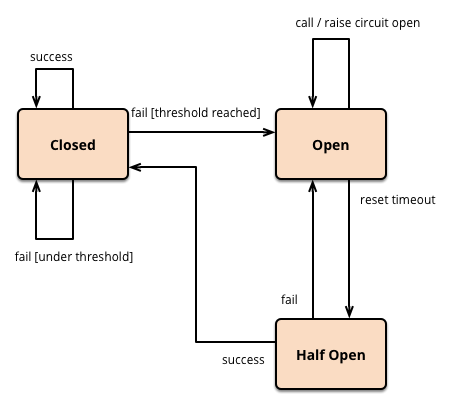
\includegraphics[width=0.5\textwidth]{circuitBreakerStates.png}
    \attribution{\url{https://martinfowler.com/bliki/CircuitBreaker.html}}
\end{center}

\begin{itemize}
    \item Closed, <<цепь замкнута>> --- все запросы направляются сервису как обычно. Если кто-то из них завершается с ошибкой, увеличивается счётчик ошибок, а если счётчик ошибок превысил допустимое значение, Circuit Breaker переходит в состояние Open.
    \item Open, <<цепь разомкнута>> --- запросы не отправляются сервису, Circuit Breaker сам выбрасывает исключение. При переходе в состояние Open запускается таймер, по истечении которого Circuit Breaker переходит в состояние Half-Open.
    \item Half-Open, <<цепь наполовину замкнута>> --- некоторое небольшое количество запросов отправляется на проксируемый сервис. Если они заканчиваются успешно, Circuit Breaker переходит в состояние Closed (и сбрасывает счётчик ошибок), иначе в Open (и перезапускает таймер).
\end{itemize}

Во время выполнения это выглядит как-то так:

\begin{center}
    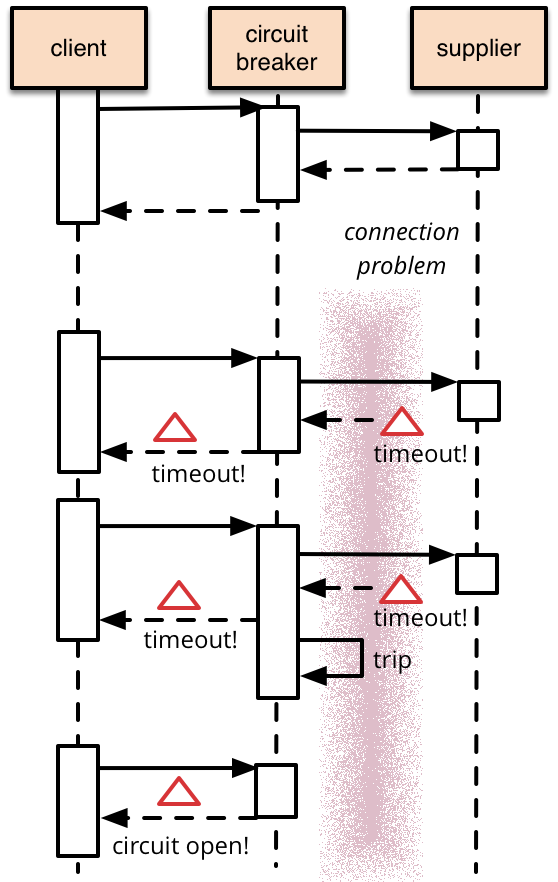
\includegraphics[width=0.35\textwidth]{circuitBreakerSequence.png}
    \attribution{\url{https://martinfowler.com/bliki/CircuitBreaker.html}}
\end{center}

Изначально всё хорошо, Circuit Breaker просто перенаправляет клиенту запросы. При возникновении проблемы Circuit Breaker получает таймаут при посылке очередного запроса и увеличивает счётчик ошибок. Если дальше всё хорошо, счётчик ошибок сбрасывается, если нет, то продолжает расти, пока не превысит порог. Как только порог превышен, Circuit Breaker переходит в разомкнутое состояние и запускает таймер. Пока таймер не отсчитает положенное время, все запросы к Circuit Breaker будут выбрасывать исключение без реальной отправки по сети.

Circuit Breaker вполне можно применять вместе с повторами, но, возможно, имеет смысл сделать механизм, позволяющий коду, выполняющему повторы, понять, что Circuit Breaker <<разомкнул цепь>> и повторы делать уже нет смысла.

\subsection{Избыточность}

Лучший способ обеспечения отказоустойчивости --- это избыточность, потому что если иметь на каждый сервис несколько его копий, при отказе одной остальные продолжат функционировать. Однако избыточность стоит денег, поэтому есть хорошие практики, позволяющие добиваться избыточности эффективно.

Во-первых, надо определиться с тем, что вы хотите от надёжности сервиса. Это чисто бизнес-решение, поскольку оно подразумевает балансировку стоимости эксплуатации и ожидаемую выгоду от надёжности системы. Так что стоит перед началом разработки определить ключевые показатели надёжности: 
\begin{itemize}
    \item Recovery Time Objective --- сколько времени должно максимум пройти с момента обнаружения отказа до восстановления системы;
    \item Recovery Point Objective --- данные за какой период до обнаружения отказа можно потерять (например, как часто надо жать на Ctrl-S при программировании, чтобы в случае падения IDE или всей системы страдать не сильно --- если раз в день, то потеряете день труда, если раз в две секунды, то две секунды, но клавиатуру испортите);
    \item Maximum Tolerable Outage --- сколько максимум времени бизнес-процесс организации может быть недоступен без значимого ущерба для организации (в отличие от RTO, MTO считает успешным восстановлением ручное исполнение бизнес-процесса).
\end{itemize}

Вот рисунок, иллюстрирующий происходящее:

\begin{center}
    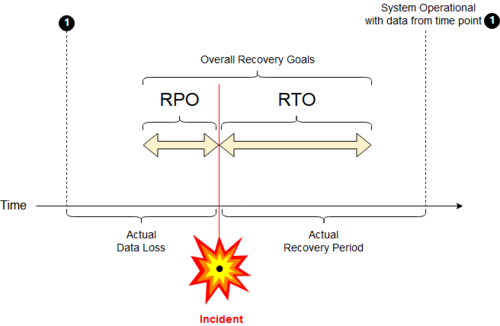
\includegraphics[width=0.5\textwidth]{rpoRtoExample.png}
    \attribution{\url{https://en.wikipedia.org/wiki/Disaster_recovery}}
\end{center}

После того, как с целевыми показателями определились, можно заложить в архитектуру механизмы их достижения.

\begin{itemize}
    \item Балансировщики нагрузки --- пожалуй, самый универсальный и надёжный инструмент. Если сервис не имеет своего состояния, запустите два (три, десять) и поставьте перед ними балансировщик нагрузки, который в случае отказа одного экземпляра просто перестаёт посылать на него запросы (впрочем, он может реализовывать более сложную логику типа Circuit Breaker). Балансировка нагрузки ещё и позитивно скажется на скорости работы системы в целом (но негативно на цене).
    \item Репликация БД --- время от времени сохранять копии базы данных (желательно в другую СУБД, готовую мгновенно включиться в работу, но можно и в снапшоты, из которых потом можно восстановить данные). Насколько часто это делать --- собственно, определяется RPO. Это абсолютно обязательная практика, так что облачными провайдерами часто делается сама собой.
    \item Разделение по регионам --- ни балансировка нагрузки, ни репликация не поможет, если всё это физически делается в одном здании, и на него упал самолёт. Все крупные и важные системы географически разнесены, что не только повышает надёжность в случае масштабных отказов, но и, опять-таки, позитивно влияет на скорость работы, при правильной настройке DNS (если пользователи автоматически направляются на ближайший к ним сервер). Очень дорого стоит.
    \item Шардирование --- техника сродни репликации, но репликация копирует всю базу, а шардирование равномерно размазывает данные по нескольким разным базам. Это сродни RAID-массиву: репликация работает как RAID 1, то есть просто копирует данные для надёжности, шардирование --- как RAID 0, то есть просто распределяет данные с целью прежде всего уменьшить время доступа к ним (операции над разными шардами всегда могут выполняться параллельно). Шардирование, тем не менее, позитивно влияет и на надёжность, поскольку в случае потери одного шарда вы теряете не все данные вообще, а только некоторые. 10\% пользователей, заказы которых вы потеряли, лучше, чем 100\% (хотя, конечно, тоже не очень, поэтому шардирование и репликация используются совместно --- пока один шард восстанавливается из резервной копии, остальные продолжают работать как ни в чём не бывало). Политика шардирования может быть разной --- можно делить записи по регионам пользователей, по первой букве из фамилии (в одной базе только фамилии на А, в другой на Б и т.п.), можно по хеш-функции от чего-нибудь, чтобы более случайно перемешать данные по шардам.
\end{itemize}

\subsection{Минимизация координации}

Компоненты распределённых приложений должны совместно работать над решением общей задачи, и если они уж слишком совместно это делают, это может нанести серьёзный ущерб производительности и надёжности системы. Поэтому с необходимостью координации действий сервисов нужно бороться, и, конечно, для этого есть несколько известных приёмов.

Первый --- использовать событийный архитектурный стиль для организации взаимодействия между сервисами. Вместо того, чтобы вызывать методы других сервисов, чтобы сообщить им, что у нас что-то произошло (например, зарегистрирован новый пользователь), можно задекларировать событие, на которое все желающие могут подписаться и асинхронно обработать. Тогда источник событий сможет даже не знать, интересно это событие кому-то или нет, или есть ли в системе другие сервисы в принципе. Такие события должны быть связаны с предметной областью, поэтому известны как доменные (domain events). Их обычно рекомендуют использовать для <<дополнительных>> сценариев (например, добавление пользователя в базу при регистрации выполняется прямым вызовом, а посылка нотификации админу --- доменным событием), но бывает так, что вся система строится только на событиях. Есть целые библиотеки, которые поддерживают такую модель, например, MediatR\footnote{Страница MediatR на GitHub: \url{https://github.com/jbogard/MediatR} (дата обращения: 12.12.2021).} для .NET.

Второй --- явно разделять команды и запросы (Command and Query Separation, CQS) и его эволюция, Command and Query Responsibility Segregation, CQRS. Идея в том, что команда должна менять состояние, но ничего не возвращать, а запрос наоборот, ничего не менять, а только возвращать текущее состояние --- и это хорошая практика в ООП вообще. CQRS делает наблюдение, что вообще говоря для команд и запросов можно использовать разные схемы БД и даже разные способы их хранения (реляционная для запросов и ООБД для команд, например), и это может в разы повысить эффективность выполнения операций. Особенно с учётом того, что при выполнении запросов не может быть конфликтов между транзакциями, раз запросы ничего не меняют. Кроме того, CQRS предполагает наличие явных доменных команд, которые содержат в себе бизнес-логику, и с которыми взаимодействуют клиенты сервиса. Разумеется, поддержание в актуальном состоянии двух разных баз с разными схемами может быть не очень простой задачей, так что реализовывать этот паттерн надо аккуратно (точнее, использовать семантику Eventual Consistency, о которой чуть дальше).

Концептуально паттерн <<CQRS>> устроен так:

\begin{center}
    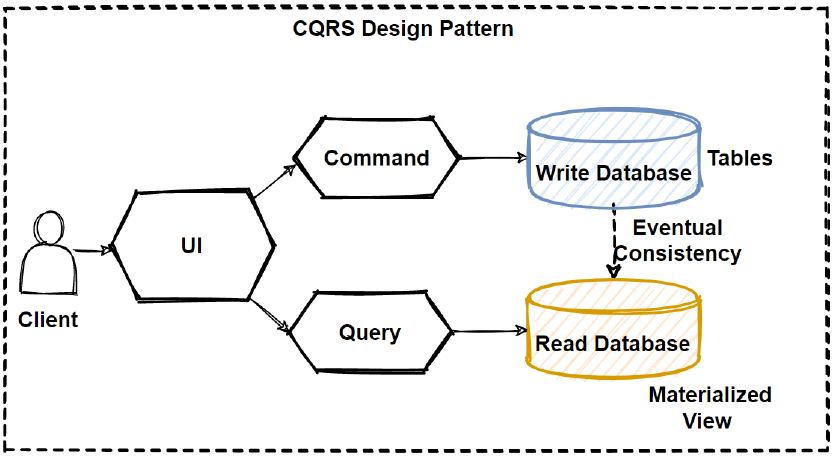
\includegraphics[width=0.8\textwidth]{cqrs.png}
    \attribution{\url{https://medium.com/design-microservices-architecture-with-patterns/cqrs-design-pattern-in-microservices-architectures-5d41e359768c}}
\end{center}

Сильно помогает, когда данные немутабельны, то есть записали один раз --- и всё. Тогда, опять-таки, конфликты при записи невозможны, есть масса возможностей для распараллеливания и эффективного хранения таких данных (вспомните Apache Kafka, она делает именно так). Это использует подход Event Sourcing --- идея его в том, что а давайте вообще не будем хранить состояние, а будем хранить только набор событий, которые в него привели. Тогда любой, кому надо, может построить текущее состояние, зная начальное и этот самый набор событий. Для скорости Event Sourcing может использовать read-only-снапшоты с текущим состоянием, которые время от времени (опять Eventual Consistency) обновляются из потока событий. Такой подход очень эффективен, когда событий много, и обработчиков много, и поддерживать между ними согласованное состояние слишком накладно (то есть на самом деле довольно часто, так что Event Sourcing нынче весьма популярен).

Наверное, не надо даже говорить, что все операции, требующие участия нескольких сервисов, должны быть асинхронными --- пока запрос выполняется, сервис должен иметь возможность делать какую-то другую работу, а не ждать ответа. Иначе может возникнуть каскад задержек, когда один сервис ждёт второй, второй --- третий и четвёртый, и т.д. Ещё на практике очень полезны так называемые \emph{идемпотентные} операции --- то есть операции, состояниекоторые могут быть повторены без изменения состояния сервера. Например, все запросы идемпотентны --- если они не меняют внутреннее состояние, от случайного повторения запроса ничего не случится. Запросы в духе <<включить>> или <<выключить>> тоже идемпотенты, потому что если мы один раз что-то включили, можем вызывать <<включить>> дальше сколько угодно раз, ничего не изменится. А вот операция <<переключить>> не идемпотентна. Идемпотентные операции хороши тем, что могут быть безопасно повторены при восстановлении после временной ошибки, и если обработчик упал, другой обработчик может просто взять очередь первого и начать последовательно выполнять операции как ни в чём ни бывало.

Шардирование данных, как, наверное, понятно, также способствует уменьшению координации, поскольку запросы не толкаются вокруг одной БД, а исполняются параллельно и не мешают друг другу.

Кстати, насчёт БД, если их несколько (что бывает почти всегда, если используется микросервисная архитектура, и очень часто в остальных случаях), поддерживать их согласованными обычно очень трудно. Есть понятие <<распределённая транзакция>>, когда хочется добиться атомарности и изолированности операции, включающей в себя несколько независимых сервисов (или независимых БД), они кажутся очень привлекательными для программистов, но их почти никто не умеет. Современная архитектурная мысль говорит, что их следует вообще избегать. Проще, быстрее и, как ни странно, надёжнее просто оптимистично выполнять операции в каждом сервисе отдельно, а если что-то пойдёт не так (например, один из участников вернёт ошибку), выполнить \emph{компенсационную транзакцию}, которая вернёт всё как было. В этом случае опять-таки используется семантика Eventual Consistency --- состояние в любой момент времени может быть несогласовано и не все сервисы могут иметь актуальные данные, но в какой-то момент в будущем гарантированно данные будут консистентны.

Это кажется не очень хорошо в плане программирования, потому что мы должны учитывать потенциальную неактуальность данных (прямо как в многопоточном программировании, где lock-free-операции должны учитывать, что данные в кеше каждого ядра могут быть свои и не соответствовать данным в памяти). Однако это суровая правда жизни, как говорит нам CAP-теорема:

\emph{В любой распределённой системе можно обеспечить не более двух из трёх свойств:
    \begin{itemize}
        \item Согласованность данных (Consistency) --- во всех вычислительных узлах данные консистентны;
        \item Доступность (Availability) --- любой запрос завершается корректно, но без гарантии, что ответы всех узлов одинаковы;
        \item Устойчивость к разделению (Partitioning Tolerance) --- потеря связи между узлами не портит корректность.
    \end{itemize}
}

Пи этом третий пункт теоремы в распределённых системах должен быть выполнен всегда, в силу принципиальной ненадёжности сети (кстати, в отличие от традиционных СУБД, которые работают на одной машине и абсолютно не устойчивы к разделению, зато гарантируют первые два пункта). Так что мы можем выбрать либо доступность, либо согласованность. Согласованность можно обеспечить, если остановить работу всех узлов, пока они не договорятся об общем состоянии (что само по себе нетривиально при возможности отказов, см., например, задачу византийских генералов\footnote{\url{https://ru.wikipedia.org/wiki/Задача_византийских_генералов} (дата обращения: 12.12.2021)}), что весьма негативно скажется на скорости работы системы (а следовательно, её доступности --- клиенты будут получать отказ в обслуживании). Доступность, однако, сама по себе тоже не очень интересна, потому что если половина серверов банка думает, что у пользователя сто рублей, а другая половина --- тысяча, это печально.

На самом деле, эта ситуация известна в теории баз данных, и есть две известные семантики работы с данными: ACID и BASE.

ACID:
\begin{itemize}
    \item Atomicity --- транзакция не применится частично;
    \item Consistency --- завершённая транзакция не нарушает целостности данных;
    \item Isolation --- параллельные транзакции не мешают друг другу;
    \item Durability --- если транзакция завершилась, её данные не потеряются.
\end{itemize}

BASE:
\begin{itemize}
    \item Basically Available --- отказ узла может привести к некорректному ответу, но только для клиентов, обслуживавшихся узлом;
    \item Soft-state --- состояние может меняться само собой, согласованность между узлами не гарантируется;
    \item Eventually consistent --- гарантируется целостность только в некоторый момент в будущем.
\end{itemize}

Семантика ACID характерна для централизованных систем, и, поскольку очень удобна в работе, её на заре интернетов пытались перенести и на распределённые приложения, однако CAP-теорема не дала. Поэтому современные распределённые приложения используют более слабую, но всё ещё полезную семантику BASE --- сервисы поддерживают целостность только своих данных и асинхронно координируются друг с другом. Собственно, Eventual Consistency, которая постоянно упоминается в этой лекции --- это часть семантики BASE.

\subsection{Проектирование для обслуживания}

Ещё один важный набор приёмов связан с тем, что распределённые приложения довольно сложно контролировать, и не всегда понятно даже, работают они или нет и что такое <<работают>> вообще (например, три секунды грузится веб-страница --- это ок или нет?). Поэтому распределённые приложения должны сразу проектироваться с учётом необходимости управлять их работой и обслуживать их во время выполнения (так называемый принцип Design for operations, основа DevOps).

Самый важный принцип в этом плане --- <<делать всё наблюдаемым>>. В частности, обеспечение логирования всего, что происходит в каждом сервисе, и централизованное отображение и анализ логов (то есть подсистема логирования внезапно сама является распределённым приложением). Как пример такой технологии см. <<Elastic Stack>>, включающую в себя такие известные штуки, как Logstash (для сбора логов), Elasticsearch (для индексации и классификации логов) и Kibana (для визуализации состояния системы по логам). В самих реализациях сервисов при этом используются библиотеки, пишущие логи (в правильно место у себя, откуда их потом заберут, или сразу в сетевое хранилище) --- log4j/slf4j и его порты и аналоги на других языках (например, log4net).

Помимо логирования есть ещё понятие <<трассировка>> --- это отслеживание того, что происходит с запросом пользователя. Трассировка, как правило, требует отслеживания обработки запроса несколькими сервисами, поэтому требуется поддержка <<корреляции>> запросов, то есть механизма, позволяющего понять, к обработке чего относится тот или иной вызов. Лог --- это как бы горизонтальный срез состояния одного сервиса, как он обрабатывает много запросов, трасса --- это как бы вертикальный срез состояния запроса, как его обрабатывают много сервисов. Трассировка позволяет локализовать отказы, идентифицировать узкие места, сетевые задержки и т.п.

На основе логов, трасс и <<counter-ов>> (то есть метрик производительности каждого конкретного сервиса) должна быть выстроена система \emph{мониторинга}, основывающаяся на численных \emph{метриках}, измеряемых в реальном времени. Примерами метрик могут быть количество обработанных запросов в секунду, количество ошибок в секунду, uptime сервисов и т.д. и т.п. Метрики специфичны для каждого конкретного приложения и определяются в основном бизнес-задачами, хотя есть и более-менее стандартные, которые измеряются оркестраторами (количество запросов, время на ответ, объём принимаемых и передаваемых данных, количество кодов HTTP 5xx в ответах, например). Организация мониторинга и выбор правильных метрик --- это в каком-то смысле искусство, но какой-то мониторинг в любом случае необходим.

Чтобы содержательный мониторинг был в принципе возможен, надо договориться о стандартном формате логов и стандартных метриках для приложения, и следить, чтобы стандартов придерживались все сервисы, из которых оно состоит. Для микросервисных приложений это само по себе может быть сложно, потому что сервисов много и они могут быть написаны на разных технологиях. Но поэтому в таких проектах грамотные архитекторы особенно полезны.

Ещё один, кажется, довольно очевидный совет --- автоматизировать всё, что может быть автоматизировано, включая развёртывание и мониторинг. Если для запуска приложения требуется четыре часа копировать куда-то файлы, запускать какие-то скрипты и руками лезть в базы, то ошибки неизбежны. В идеале всё, что делается с приложением, должно делаться автоматически одной командой.

Этого можно добиться, если относиться к конфигурации приложения, как к коду, который можно хранить, версионировать, согласованно редактировать и автоматически применять в рамках обычного CI/CD-процесса. Этому принципу следуют популярные оркестраторы, такие как Docker Compose и Kubernetes (про которые чуть позже) --- в конфигурации оркестратора (обычно в виде YAML или JSON-файлов) описывается, какие сервисы в скольки экземплярах на каких портах должны быть запущены, кто раньше, кто позже, у кого какая конфигурация (задаваемая, например, через переменные окружения) и что делать, если кто-то упал. Конфигурация выкладывается в систему контроля версий и применяется одной командой (docker compose up или kubectl apply), лезть в конфигурацию работающей системы руками (например, чтобы остановить или запустить сервис) считается чем-то плохим.

\end{document}